%% =============================================================================
%% ОБЩИЕ ПРАВИЛА (для людей и для ИИ-агентов)
%% =============================================================================
%% 1. Это черновик ОДНОГО участника. Редактируй только этот файл.
%% 2. Не меняй чужие файлы в папке drafts/.
%% 3. Не трогай корневой main.tex, преамбулу, стили (.cls, .sty), .github/.
%% 4. Можно использовать существующие метки (ef, \label, \cite), но не переименовывай их без согласования.
%% 5. Новые рисунки складывай в figures/ с уникальным именем: <имя>_<смысл>.png.
%% 6. Новые источники (BibTeX) пришли Давиду (david_final.tex) или в issues.
%% 7. Сохраняй статью в формате IEEEtran; не меняй шрифты/поля.
%% 8. После правки скинь файл координатору; сборка PDF делается в main.tex.
%% =============================================================================

%% УЧАСТНИК: Юра
%% РАЗДЕЛЫ: AI and standards + Problems and state of the art + описания ISA-88/95/5.1
%% ЗАДАЧИ:
%%   - Переформулировать все тезисы про стандарты и онтологии.
%%   - Привязать ISA-88/95/5.1 к задаче пастеризации (рецепты, MES/ERP, документация).
%%   - Обновить TikZ-диаграммы ISA (цвета/формы) или заменить на новые схемы.
%%   - Добавить свежие источники по ISA и онтологиям (2023-2025).
%% =============================================================================

\section{AI and standards}

Deep learning has produced controllers that approximate process dynamics with
high accuracy. Such controllers answer only \emph{what} to do next, never
\emph{why}. A systematic review of 167 papers reports that explainability and
trustworthiness remain the least developed aspects of the field
\cite{Colelough2025}. Neuro-symbolic AI closes this gap by coupling statistical
learning with an explicit symbolic model of the domain. For a pasteurization
unit the distinction is practical: a neural regulator may propose a new
setpoint, but the operator must be able to trace that setpoint back to the
recipe, the equipment, and the safety limits that justify it.

Standardization fixes the concepts, terminology, typology, and reference models
of a mature engineering activity. It also prescribes the documents that
accompany design, commissioning, and operation. Standards therefore address the
\textbf{compatibility problem}, which is central to every rapidly evolving
information technology \cite{Golenkov2019}. Compatibility must hold at several
levels simultaneously: the terminology shared by the parties, the data exchanged
between their tools, and the sequence of actions each party performs.

The same requirement reappears in digital twin engineering, where one plant is
described by many heterogeneous and independently authored models. Joining these
models into a single twin demands conceptual unification rather than another
data converter \cite{DigitalTwins}. Modern SCADA platforms face the same
pressure towards integration, scalability, and vendor independence
\cite{Mladen2022}.

Most standards, however, are still published as linear documents or as sets of
static web pages connected by hyperlinks. This form hides the structure of the
standard behind prose and forces every reader to reconstruct that structure
mentally. The overhead of maintaining and applying the standard then grows until
it outweighs the benefit the standard was meant to deliver \cite{Serenkov-2004}.

Semantic technologies permit a different form, in which a standard is
represented as formalized knowledge that an intelligent system processes
directly. An ontology fixes the vocabulary of a domain together with the
relations between its concepts, which gives people and programs one shared
interpretation \cite{Golenkov2019}. Industrial automation has already taken this
route: ISA-88 and ISA-95 have been reconstructed as an ontology network for
planning and scheduling \cite{Vegetti2022}, as the schema of an industrial
knowledge graph \cite{Listl2023}, and as input to a unified manufacturing
operations management ontology aligned with the Industrial Ontology Foundry
\cite{Sarkar2026}.

ISA has itself moved towards machine processing of its content with Mimo, a
large language model (LLM) trained on ISA standards, technical reports, and
related material \cite{Mimo2024}. Mimo explains provisions and answers questions
in natural language, yet it is closed source and cannot be embedded into a
control loop. An LLM also reproduces the wording of a standard without
guaranteeing that a generated action satisfies it. Work on regulated process
automation argues for the opposite arrangement, in which symbolic constraints
become architectural components of the agent and violations are structurally
impossible \cite{Rombach2026}. That arrangement is the one pursued below for the
pasteurization unit.

\section{Problems and state of the art}

Published analyses of standardization practice \cite{Serenkov-2004, Uglev-2012}
converge on four problems, all rooted in the document form of a standard rather
than in its content:

\begin{itemize}
  \item \emph{Redundancy.} The same notion is restated in several parts of the
    standard and in the documents that reference it, so a change of terminology
    must be propagated by hand.
  \item \emph{Internationalization.} A translated standard becomes an
    independent version that has to be kept synchronized with the original.
  \item \emph{Retrieval.} Locating the provision that applies to a given piece
    of equipment requires reading the surrounding prose, which makes both study
    and daily use expensive.
  \item \emph{Verification.} Checking that an object or a procedure conforms to
    a standard cannot be automated while the requirements exist only as text.
\end{itemize}

On a pasteurization unit these costs are concrete. The same vessel is named one
way in the SCADA project, another way in the EPLAN documentation, and a third
way in the MES production order. Reconciling the three descriptions is manual
work that repeats after every modernization of the unit.

The most promising remedy is to transform each standard into a knowledge base
built on the ontologies of that standard \cite{Golenkov2019, Serenkov-2004,
Uglev-2012, Improving-2017, ISA-88-formalization}. Development and application
of the standard then become operations over knowledge instead of operations over
text. Three ISA standards govern the pasteurization unit;
Table~\ref{tab:isa_parts} summarizes their parts and their role in the project.

\begin{table}[ht]
  \caption{ISA standards applied to the pasteurization unit}
  \label{tab:isa_parts}
  \centering
  \small
  \begin{tabular}{@{}p{0.14\columnwidth}p{0.34\columnwidth}p{0.38\columnwidth}@{}}
    \hline
    Standard & Principal parts & Role in the project \\
    \hline
    ISA-88 \cite{ISA88} & 88.00.01--2010, 88.00.02--2001, 88.00.03--2003,
    88.00.04--2006, IEC 61512-1 & Physical and procedural models of batch
    production: recipes, units, and equipment modules \\
    ISA-95 \cite{ISA95} & 95.00.01--2010 through 95.00.08--2020 & Boundary
    between control and business systems; exchange with MES and ERP \\
    ISA-5.1 \cite{ISA_5_1} & 5.1--2024, TR 5.1.02--2024, TR 5.1.03--2024,
    5.06.01--2007 & Symbols and identification of instrumentation on diagrams
    and in project documentation \\
    \hline
  \end{tabular}
\end{table}

\subsection{ISA-88 and the pasteurization unit}

ISA-88 \cite{ISA88} separates what is produced from the equipment that produces
it. Its physical model decomposes a plant into enterprise, site, area, process
cell, unit, equipment module, and control module. Its procedural model
decomposes a recipe into procedure, unit procedure, operation, and phase. A
recipe is written against the procedural model and bound to the physical model
only at execution time, so a change of formulation does not require rewriting
the control program.

Fig.~\ref{fig:yura_s88_pasteurizer} applies both models to the pasteurization
unit. The pasteurizer is a unit inside the process cell of the dairy production
area. Its equipment modules are the heater node, the holding section, the cooler
node, and the shared clean-in-place (CIP) line, whereas individual valves,
pumps, and temperature transmitters are control modules. The unit procedure of a
pasteurization batch consists of four operations: filling, heating to the
holding temperature, holding, and cooling. The CIP procedure reuses the same
physical objects under a different recipe, which is exactly the reuse ISA-88 is
designed to enable.

\begin{figure}[ht]
  \centering
  \begin{adjustbox}{width = \columnwidth}
    \begin{tikzpicture}[node distance=5mm and 10mm, every node/.style={draw, rounded corners, align=center, minimum width=34mm, minimum height=7mm, fill=blue!12}, arrow/.style={-Latex, thick}]
      \node[fill=blue!28] (cell) {Process cell:\\dairy production area};
      \node[below=of cell] (unit) {Unit:\\pasteurizer};
      \node[below=of unit] (em) {Equipment modules:\\heater, holding section,\\cooler, CIP line};
      \node[below=of em] (cm) {Control modules:\\valves, pumps,\\temperature transmitters};

      \node[fill=blue!28, right=of cell] (proc) {Unit procedure:\\pasteurization batch};
      \node[below=of proc] (op) {Operations: filling,\\heating, holding, cooling};
      \node[below=of op] (ph) {Phases: open valve,\\ramp setpoint,\\hold 15 s at 72~$^{\circ}$C};
      \node[below=of ph] (cmd) {Commands issued\\to control modules};

      \draw[arrow] (cell) -- (unit); \draw[arrow] (unit) -- (em); \draw[arrow]
      (em) -- (cm); \draw[arrow] (proc) -- (op); \draw[arrow] (op) -- (ph);
      \draw[arrow] (ph) -- (cmd); \draw[arrow, dashed] (cmd) -- (cm);
    \end{tikzpicture}
  \end{adjustbox}
  \caption{ISA-88 physical and procedural models instantiated for the
  pasteurization unit}
  \label{fig:yura_s88_pasteurizer}
\end{figure}

\subsection{ISA-95 and the MES/ERP boundary}

ISA-95 \cite{ISA95} describes the interface between production control and
business planning. It arranges an enterprise into five levels, from the sensors
and actuators of level 0 to the business planning of level 4, and fixes the
information crossing each boundary \cite{ISA95_Siemens}. The critical boundary
lies between level 2, where the pasteurization unit is controlled in real time,
and level 3, where batches are scheduled and reported. This model is usable
directly as the schema of an industrial knowledge graph rather than only as a
documentation convention \cite{Listl2023}.

Fig.~\ref{fig:yura_isa95_levels} places the OSTIS knowledge base on that
boundary. The knowledge base stores the ISA-88 recipes and the equipment model
of the unit, receives production orders from the MES, and returns batch reports
and process indicators. The neuro-symbolic controller reads its setpoints from
the same knowledge base. Consequently the recipe scheduled by the business
system and the recipe executed by the controller are one object rather than two
synchronized copies.

\begin{figure}[ht]
  \centering
  \begin{adjustbox}{width = \columnwidth}
    \begin{tikzpicture}[lvl/.style={draw, rounded corners, align=center, minimum width=58mm, minimum height=8mm, fill=green!12}, kb/.style={draw, rounded corners, align=center, minimum width=36mm, minimum height=16mm, fill=green!28}, arrow/.style={-Latex, thick}]
      \node[lvl] (l4) at (0,4.4) {Level 4: business planning (ERP)};
      \node[lvl] (l3) at (0,3.3) {Level 3: manufacturing operations (MES)};
      \node[lvl] (l2) at (0,2.2) {Level 2: supervisory control (SCADA)};
      \node[lvl] (l1) at (0,1.1) {Level 1: sensing and actuation (PLC)};
      \node[lvl] (l0) at (0,0.0) {Level 0: the pasteurization unit};

      \node[kb] (kb) at (6.4,2.75) {OSTIS knowledge base:\\ISA-88 recipes,\\equipment model};

      \draw[arrow] (l4) -- (l3); \draw[arrow] (l3) -- (l2); \draw[arrow] (l2) --
      (l1); \draw[arrow] (l1) -- (l0);

      \draw[arrow] (l3.east) -- node[above, font=\footnotesize] {production
      order} (kb.north west);
      \draw[arrow] (kb.south west) -- node[below, font=\footnotesize]
      {setpoints, batch report} (l2.east);
    \end{tikzpicture}
  \end{adjustbox}
  \caption{Place of the OSTIS knowledge base at the ISA-95 level 2--3 boundary}
  \label{fig:yura_isa95_levels}
\end{figure}

\subsection{ISA-5.1 and project documentation}

ISA-5.1 \cite{ISA_5_1} governs the third face of the same plant, its
documentation. The standard fixes the symbols and tag identifiers of
instrumentation on process and instrumentation diagrams, so that a temperature
transmitter carries one designation in the drawing, in the wiring documentation,
and in the control program. The scope of the ISA5 committee is broader than the
diagrams alone: it covers recommended practices and technical reports for
documenting measurement and control systems in any industry. On the
pasteurization unit this notation is generated by EasyEPLANner
\cite{EasyEPLANner}, an add-in that derives the device description from the
EPLAN project.

Formalizing the three standards yields a set of interconnected subject domains
rather than three independent glossaries (Fig.~\ref{fig:yura_ontologies}). The
subject domain of physical models of batch manufacturing enterprises supplies
the ISA-88 hierarchy from process cell to control module. The subject domain of
devices supplies the instrument classes of ISA-5.1, and the two domains share
the objects that ISA-95 reports to the MES. The corresponding knowledge bases
are developed as open projects \cite{s88-ostis, isa-5.1-ostis} and continue the
ontological design of prescription production described in \cite{Taberko2017}.

\begin{figure}[ht]
  \centering
  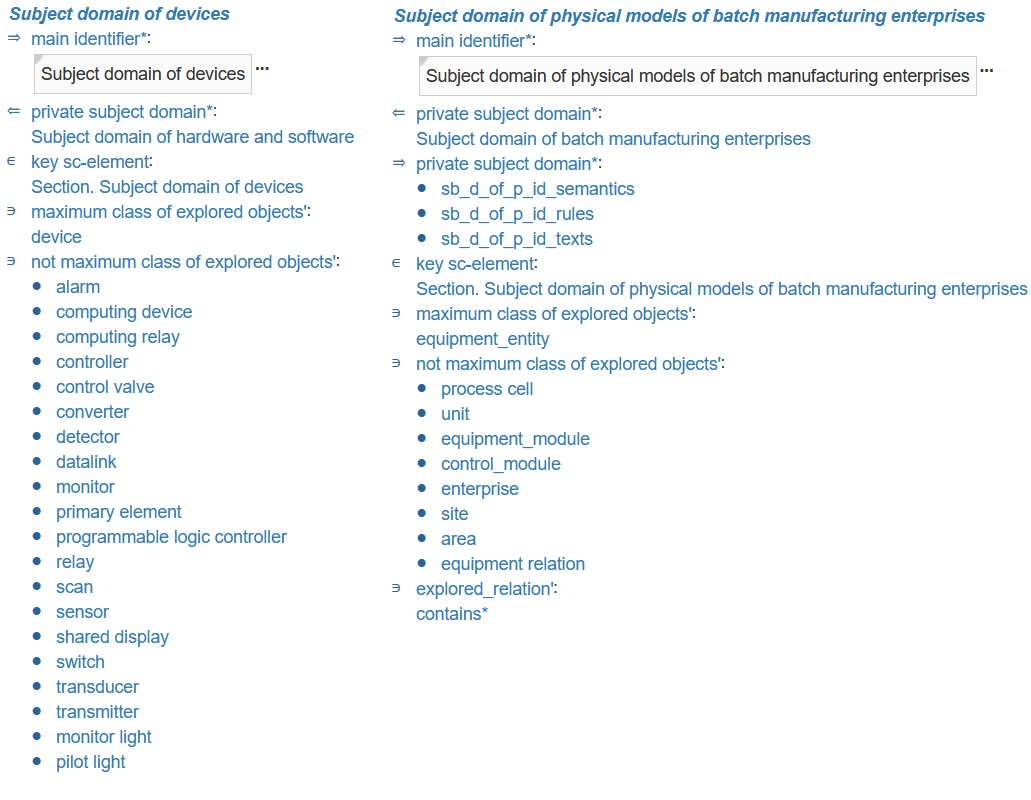
\includegraphics[width=\columnwidth]{figures/pic_resulting_ontologies.png}
  \caption{Subject domains obtained by formalizing ISA-88 and ISA-5.1}
  \label{fig:yura_ontologies}
\end{figure}

%% =============================================================================
%% НОВЫЕ ИСТОЧНИКИ — ДЛЯ ДАВИДА (перенести в bib/links.bib)
%% Метаданные сверены по arXiv / Crossref / NIST.
%% Пока записи не добавлены, bibtex выдаёт warning и печатает [?] вместо
%% номера; сборка при этом не падает.
%% =============================================================================
%
% @misc{Colelough2025,
%   author       = {Brandon C. Colelough and William Regli},
%   title        = {Neuro-Symbolic {AI} in 2024: A Systematic Review},
%   year         = {2025},
%   howpublished = {\url{https://arxiv.org/abs/2501.05435}},
%   note         = {arXiv:2501.05435}
% }
%
% @article{Vegetti2022,
%   author  = {Marcela Vegetti and Gabriela Henning},
%   title   = {Ontology network to support the integration of planning and scheduling activities in batch process industries},
%   journal = {Journal of Industrial Information Integration},
%   volume  = {25},
%   pages   = {100254},
%   year    = {2022},
%   doi     = {10.1016/j.jii.2021.100254}
% }
%
% @article{Listl2023,
%   author  = {Franz Georg Listl and Jan Fischer and Annelie Sohr and Daniel Dittler and Nasser Jazdi and Michael Weyrich},
%   title   = {Utilizing {ISA-95} in an Industrial Knowledge Graph for Material Flow Simulation --- Semantic Model Extensions and Efficient Data Integration},
%   journal = {Procedia CIRP},
%   volume  = {120},
%   pages   = {1558--1563},
%   year    = {2023},
%   doi     = {10.1016/j.procir.2023.09.214}
% }
%
% @inproceedings{Sarkar2026,
%   author    = {Arkopaul Sarkar and Boonserm Kulvatunyou and Evan Wallace and Milos Drobnjakovic and Gabriela Henning and Ana Nikolov and Saruda Seeharit and Dusan Sormaz and Adlene Rebai and Yan Lu},
%   title     = {Toward a Standardized Manufacturing Operation Management Ontology ({MOMO}): Findings from the {NIST} Workshop},
%   booktitle = {28th International Conference on Production Research (ICPR-28)},
%   series    = {Lecture Notes in Production Engineering},
%   publisher = {Springer},
%   year      = {2026}
% }
%
% @misc{Rombach2026,
%   author       = {Alexander Rombach and Chantale Lauer and Nijat Mehdiyev},
%   title        = {Neuro-Symbolic Agents for Regulated Process Automation: Challenges and Research Agenda},
%   year         = {2026},
%   howpublished = {\url{https://arxiv.org/abs/2606.13405}},
%   note         = {arXiv:2606.13405}
% }
%
%% =============================================================================
